  \section{Nodes}
  \subsection{Set up}
    \begin{enumerate}
      \item Ensure the node is plugged in to an outlet, and the switch is in the \textbf{ON} position 
      (it should be ON by default).
      The red light will be illuminated on the node when it is on.\\ 
TODO ADD GRAPHIC NODE ON\\
      \begin{center}
      
\includegraphics[scale=1]{images/Now-Later.png}
    \end{center}

      If the node has already been activated, you are done with this section, proceed to the Web section (Part 3).

      \item If this is the first time the node is being connected to the hub,
      you will need to activate it. To do this you will need a device
      capable of connecting to a wifi network, such as a smart phone, tablet, or computer.\\
      \\ 
      Under wifi networks, you should see a network called \textbf{SetUpGadget\_FPFDHI}\\
      Note that the "FPFDHI" can be any sequence of letters and is specific to the node. Connect to that network. 
      \emph{Once connected you may get a warning that the network does not have access
      to the internet. That is normal, proceed anyway.}

      \item Open your browser and navigate to \textbf{192.168.4.1}

      \begin{center}
      
\includegraphics[scale=1]{images/ip-enter.png}
    \end{center}  

      This will bring up a wifi login page:

      \begin{center}
      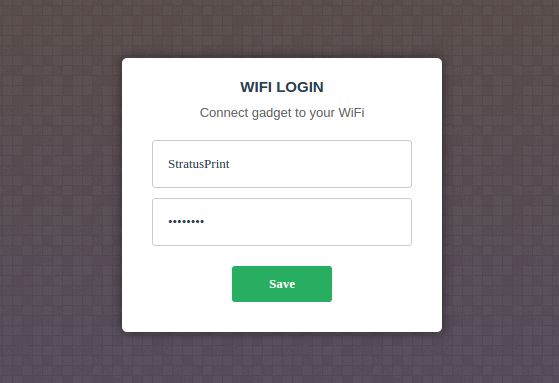
\includegraphics[scale=0.25]{images/wifi-login.png}
    \end{center}
      Type the information as follows (\emph{case matters, use both upper- and lower-case letters as indicated}):\\
      The wifi name is \textbf{StratusPrint}\\ 
      The password is \textbf{FusRoDah}\\
      \emph{This is the default wifi name and password for the hub and can be changed later.}\\


      \item Click the save button. If successful, the \textbf{SetUpGadget\_FPFDHI} network should disappear
      from your visible networks. This may take 1-3 minutes. If the network is still
      visible, please turn your wifi off and on again to confirm it remains visible. If it is still there,
      please start over from step 2 and make sure you correctly input all information.

    \end{enumerate}

  \subsection{Sensors}
  \emph{This section provides more information on the sensors currently attached to the node, and 
      how to add new sensors.  You may skip this section if you are not adding or replacing sensors.}\\
  \subsubsection{Node Pinout}
  \begin{center}
        \includegraphics[scale=0.05]{images/node-pin-out.png}
  \end{center}
    \subsubsection{Job Button}
      The "Job Button" indicates when a job is complete, and starts a new job when pressed. This provides an easy way
      for a user to know when a job is completed.\\

      \textbf{Operation}\\
      Once a print is complete this button will blink repeatedly until it is pressed.  Remove the completed project,
      clean the print bed, then press the button to start the next job in the print queue.\\

      \textbf{Wiring Diagram}\\
            \begin{center}
      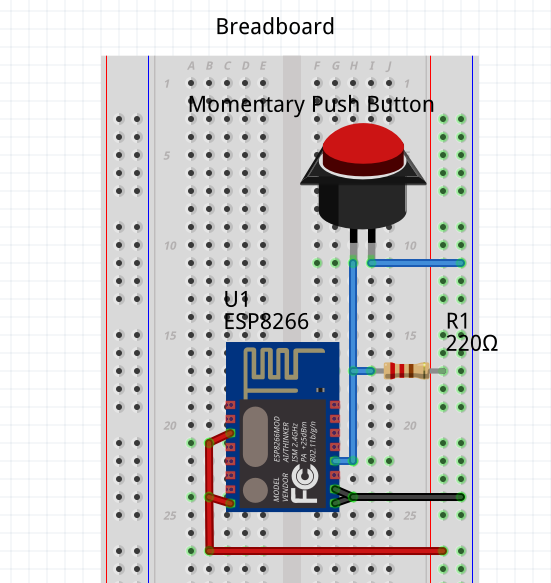
\includegraphics[scale=0.25]{images/job-cir.png}
      \end{center}
    \subsubsection{Temperature and Humidity}
      The temperature and humidity sensor will report the current room conditions. It
      can detect dangerous conditions for 3D printing and act as an early warning system
      if the conditions may lead to print errors.\\

      \textbf{Wiring Diagram}\\
            \begin{center}
      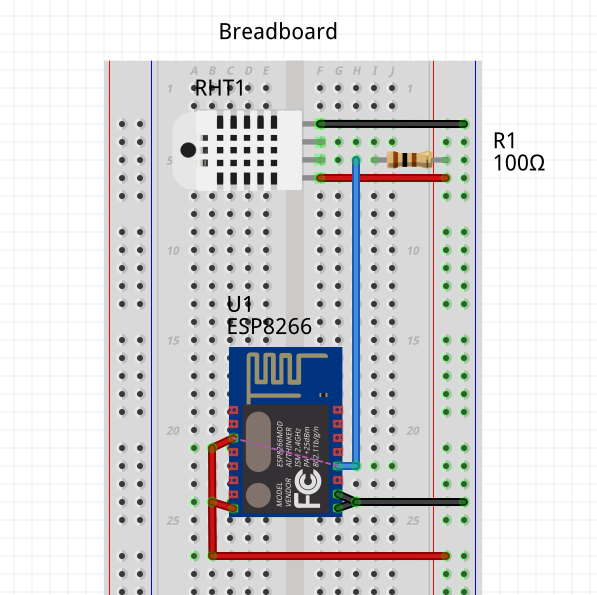
\includegraphics[scale=0.25]{images/temp-diagram.png}
\end{center}

    \subsubsection{Door Sensor}
      The door sensor is a magnetic switch mounted to the entrance of the printing lab.
      This allows for detection of an open or closed door, which may affect printing conditions.\\

      \textbf{Wiring Diagram}\\
      \begin{center}
        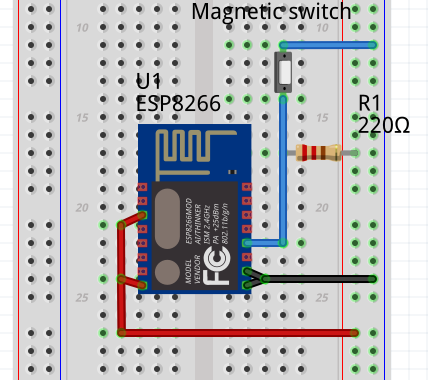
\includegraphics[scale=0.25]{images/door-cir.png}
        \end{center}
    \subsubsection{Additional Sensors}
      The nodes were set up to be universal, therefore they are compatible with
      many sensors. The nodes come with a breadboard so they can
      easily be reconfigured.\\
\newpage
  \subsection{Troubleshooting}
  \subsubsection{Reset}
  Turn the switch the the off position and unplug the node.
  \subsubsection{Node is not connecting to the hub}
  \begin{enumerate}
    \item Ensure the node has the correct wifi credentials. If the default is not
    working make sure the password hasn't been changed.
    \item If the node seems to be connected and isn't communication hard reset and re-connect.
  \end{enumerate}
  \subsubsection{Node is connected but no data is being sent from the sensors}
  Make sure the sensors are connected correctly you can reference the wiring diagrams
  in this manual.
